\documentclass[a4paper]{article}

\usepackage{amsmath, blindtext, float, graphicx, hyperref}
\graphicspath{ {./images/} }
\title{Bayesian Deep Leaning and a Probablistic Perspective of Generalization}
\author{Shubham Gupta}

\begin{document}
\maketitle
\section{Introduction}
\begin{itemize}
    \item I found this paper from Andrew Gordon Wilson's twitter account(@andrewgwils) and the tweet/summary is available \href{https://twitter.com/andrewgwils/status/1230669857840123906}{here}
    \item This is another paper following the recent discussion around Bayesian Deep Learning, and I only decided to read this for fun!
\end{itemize}
\section{Paper Introduction}
\begin{itemize}
    \item Parameter count is a poor indicator of generalization ability.
    \item Generalization depends on:
    \begin{itemize}
        \item Support
        \item Inductive biases of a model
    \end{itemize}
    \begin{figure}[H]
        \centering
        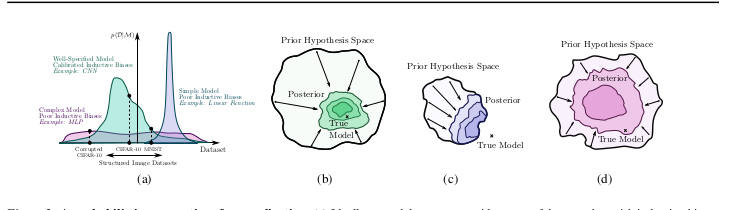
\includegraphics[width=0.8\textwidth]{prob_perspective}
        \caption{Probabilistic Perspective on Generalization}
        \label{fig:prob_perspective}
    \end{figure}
    \item For the given evidence(marginal likelihood), we have: $p(D|M) = \int p(D|M, w)p(w)dw$
    \item \textit{Support} is: p(D|M) > 0
    \item \textit{Inductive Biases}: Relative prior probabilities of diffrent datasets i.e distribution of support given by p(D|M)
\end{itemize}

\end{document}
